\subsection{OB-18 (HWB)}
Kontaktní a bezkontaktní čipové karty, princip činnosti a použití. Radiofrekvenční identifikace (RFID) a komunikace v blízkém poli (NFC).

\subsubsection*{Čipové karty obecně}
\begin{itemize}
	\item obvykle plastové kartičky obsahující integrovaný obvod
	\item obecněji --- nosič informace a bezpečnostních funkcí
	\item odolnost proti padělání
	\item lze použít např. pro vícefaktorovou autentizaci
	\item obsahuje vlastně počítač, který je: konfigurovatelný pomocí API, programovatelný při výrobě nebo i v térénu (java karty)
	\item z čeho se skládá: výpočetní jednotky (CPU, kryptografický koprocesor), paměti (RAM, ROM, EEPROM), komunikační zařízení, obvody napájení, senzory
\end{itemize}

\subsubsection*{Kontaktní karty}
\begin{itemize}
	\item rozhraní / konektor má typicky 6 nebo 8 pinů
	
	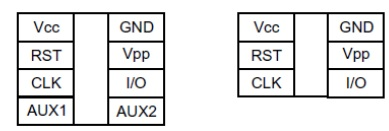
\includegraphics[width=0.4\textwidth]{img/OB-18_0.jpg}
	
	\item Inicializace připojení
	\begin{itemize}
		\item indikace přítomnosti karty
		\item zapnutí napájení
		\item signál hodin, reset
		\item karta pošle odpověď na reset (ATR --- Answer to Reset)
		\item dekódování ATR
		\item volba parametrů protokolu
	\end{itemize}
	\item přenos dat APDU (Application Protocol Data Unit --- něco jako aplikační vrstva) pomocí TPDU (Trans\-mission Protocol Data Unit --- něco jako transportní vrstva)
	\item T=0 --- byte oriented protocol
	\item T=1 --- block oriented protocol
\end{itemize}

\subsubsection*{Bezkontaktní karty}
\begin{itemize}
	\item zajímá nás hlavně norma ISO 14443 (vysoká frekvence --- 13.56MHz, komunikace na blízko), je používána často, jako v platebních kartách, lítačka, pas, průkaz ČVUT...
	\item RFID (RadioFrekvenční Identifikace)
	\begin{itemize}
		\item systém, který používá elektromagnetické pole k automatické identifikaci a sledování transponderů připevněných k objektům
		\item můžou se přenášet jak data tak napájení
		\item transponder --- nosič dat připevněný k objektu --- anténa + mikročip
		\item čtečka --- napájí a komunikuje s transpondery --- RF modul + řídící jednotka + anténa
	\end{itemize}
	\item NFC (Near FIeld Communication)
	\begin{itemize}
		\item rozšiřuje technologii RFID na bezdrátové datové rozhraní mezi zařízeními
		\item sada komunikačních protokolů pro přenos dat mezi dvěma zařízeními na krátkou vzdálenost (do cca 4 cm)
		\item pasivní transponder --- nemá baterii/zdroj napájení, všechna energie čerpána z čtečky
		\item aktivní transponder --- obsahuje baterii
		\item využití: bezkontaktní platební systémy, sdílení dat, elektronický průkaz, vstupní karta...
	\end{itemize}		 
\end{itemize}